%%%%%%%%%%%%%%%%%%%%%%%%%%%%%%%%%%%%%%%%%
% University Assignment Title Page 
% LaTeX Template
% Version 1.0 (27/12/12)
%
% This template has been downloaded from:
% http://www.LaTeXTemplates.com
%
% Original author:
% WikiBooks (http://en.wikibooks.org/wiki/LaTeX/Title_Creation)
%
% License:
% CC BY-NC-SA 3.0 (http://creativecommons.org/licenses/by-nc-sa/3.0/)
% 
% Instructions for using this template:
% This title page is capable of being compiled as is. This is not useful for 
% including it in another document. To do this, you have two options: 
%
% 1) Copy/paste everything between \begin{document} and \end{document} 
% starting at \begin{titlepage} and paste this into another LaTeX file where you 
% want your title page.
% OR
% 2) Remove everything outside the \begin{titlepage} and \end{titlepage} and 
% move this file to the same directory as the LaTeX file you wish to add it to. 
% Then add \input{./title_page_1.tex} to your LaTeX file where you want your
% title page.
%
%%%%%%%%%%%%%%%%%%%%%%%%%%%%%%%%%%%%%%%%%
%\title{Title page with logo}
%----------------------------------------------------------------------------------------
%   PACKAGES AND OTHER DOCUMENT CONFIGURATIONS
%----------------------------------------------------------------------------------------

\documentclass[12pt]{article}
\usepackage[english]{babel}
\usepackage[utf8x]{inputenc}
\usepackage{amsmath}
\usepackage{graphicx}
% \usepackage[colorinlistoftodos]{todonotes}

\begin{document}

\begin{titlepage}

\newcommand{\HRule}{\rule{\linewidth}{0.5mm}} % Defines a new command for the horizontal lines, change thickness here

\center % Center everything on the page
 
%----------------------------------------------------------------------------------------
%   HEADING SECTIONS
%----------------------------------------------------------------------------------------

\textsc{\LARGE Universidade Federal de Ciências da Saúde de Porto Alegre}\\[1.5cm] % Name of your university/college
\textsc{\Large Informática Biomédica }\\[0.5cm] % Major heading such as course name
\textsc{\large Disciplina de Verificação e Validação de Software}\\[0.5cm] % Minor heading such as course title

%----------------------------------------------------------------------------------------
%   TITLE SECTION
%----------------------------------------------------------------------------------------

\HRule \\[0.4cm]
{ \huge \bfseries Plano geral de teste do software HospitalRun}\\[0.4cm] % Title of your document
\HRule \\[1.5cm]
 
%----------------------------------------------------------------------------------------
%   AUTHOR SECTION
%----------------------------------------------------------------------------------------

\begin{minipage}{0.4\textwidth}
\begin{flushleft} \large
\emph{Aluno:}\\
Nicolas Zachow Coelho
\end{flushleft}
\end{minipage}
~
\begin{minipage}{0.4\textwidth}
\begin{flushright} \large
\emph{Professora:} \\
Juliana Herbert
\end{flushright}
\end{minipage}\\[2cm]

% If you don't want a supervisor, uncomment the two lines below and remove the section above
%\Large \emph{Author:}\\
%John \textsc{Smith}\\[3cm] % Your name

%----------------------------------------------------------------------------------------
%   DATE SECTION
%----------------------------------------------------------------------------------------

% {\large \today}\\[2cm] % Date, change the \today to a set date if you want to be precise
{\large 2016/2}\\[2cm] % Date, change the \today to a set date if you want to be precise

%----------------------------------------------------------------------------------------
%   LOGO SECTION
%----------------------------------------------------------------------------------------


\includegraphics[scale=0.5]{logo.jpg}\\[1cm] % Include a department/university logo - this will require the graphicx package
 
%----------------------------------------------------------------------------------------

\vfill % Fill the rest of the page with whitespace

\end{titlepage}


\tableofcontents

\newpage

\section*{Histórico de alterações}

\subsection*{Controle de configuração}

\begin{table}[h]
\centering
\begin{tabular}{|l|l|}
 \hline
\textbf{Título} & Plano geral de teste do software \textbf{HospitalRun} \\\hline
\textbf{Autor} & Nicolas Zachow Coelho \\\hline
\textbf{Última alteração} & \today  \\\hline
\end{tabular}
\end{table}


\subsection*{Histórico de documentação}

\begin{table}[h]
\centering
\begin{tabular}{|l|l|l|}
 \hline
    \textbf{Versão} &  \textbf{ Data } & \textbf{Conteúdo} \\\hline
    1.0 & 23/08/16 & Versão inicial \\\hline
    1.1 & 26/08/16 & Mudança para o \LaTeX \\\hline
    1.2 & 27/08/16 & Análise geral e análise de dominio (ID) \\\hline
\end{tabular}
\end{table}

\newpage

\section*{Resumo executivo}
\addcontentsline{toc}{section}{\protect\numberline{}Resumo executivo}
Este plano de teste tem o objetivo de documentar as atividades de teste
funcional de software realizadas durante a disciplina de “Validação e
Verificação de Software na Área da Saúde”.

Com base nesta documentação, pretende-se:
\begin{itemize}
\item determinar o esforço necessário para as atividades a serem realizadas;
\item compartilhar informações sobre as atividades de teste de software, dentro
    e fora da equipe de teste;
\item direcionar as atividades da equipe de teste em direção a um objetivo comum;
\item documentar aspectos importantes do teste de software, tais como
    estratégia, técnicas e casos de teste, entre outros.
\end{itemize}

\section*{Caracterização do software}
\addcontentsline{toc}{section}{\protect\numberline{}Caracterização do software}
HospitalRun é um projeto OpenSource realizado com a intenção de entregar
software moderno para unidades de saude de paises subdesenvolvidos.
Ele foi desenvolvido para ser utilizado diretamento no browser. Além disto ele
também foi projeto com a realidade de conexões de internet precárias em mente,
possibilitando que ele seja utilizado mesmo sem conexão.
\\
http://hospitalrun.io/


\section*{Visão geral da funcionalidade do software}
\addcontentsline{toc}{section}{\protect\numberline{}Visão geral da funcionalidade do software}
O software permite o controle completo de uma unidade de saúde.

\begin{itemize}
\item Gerenciamento de pacientes
\item Gerenciamento de exames
\item Gerenciamento de estoque
\end{itemize}

\section*{Seleção das funções a serem testadas}
\addcontentsline{toc}{section}{\protect\numberline{}Seleção das funções a serem testadas}
Escolhemos o módulo de gerenciamento de pacientes para realizar os testes.
Esta escolha é praticamente imediata, já que um problema nesta parte do
software pode comprometer todo o resto do software.

\section*{Definição dos riscos para o teste}
\addcontentsline{toc}{section}{\protect\numberline{}Definição dos riscos para o teste}
Esse software está mais ligado a área de administração do que à área da saúde,
por isso seus riscos não são tão grandes.

Um dos piores problemas é a perda de informação sobre pacientes ou exames mas
isso é facilmente contornável utilizando-se de uma solução de backup
independente.

Um problema mais grave é o vazamento de informações. Este é um risco real e com
uma probabilidade alta de acontecer.

\section*{Descrição do ambiente de teste}
\addcontentsline{toc}{section}{\protect\numberline{}Descrição do ambiente de teste}
Os testes serão realizados em uma máquina com o Fedora 24, utilizando a ultima
versão estável disponível do Firefox(47.0-4.fc24).

\section*{Restrições do teste}
\addcontentsline{toc}{section}{\protect\numberline{}Restrições do teste}
Ainda não projetamos nenhuma restrição para os testes, mas elas certamente
aparecerão no futuro.

\section*{Análise geral da variáveis}
\addcontentsline{toc}{section}{\protect\numberline{}Análise geral da variáveis}
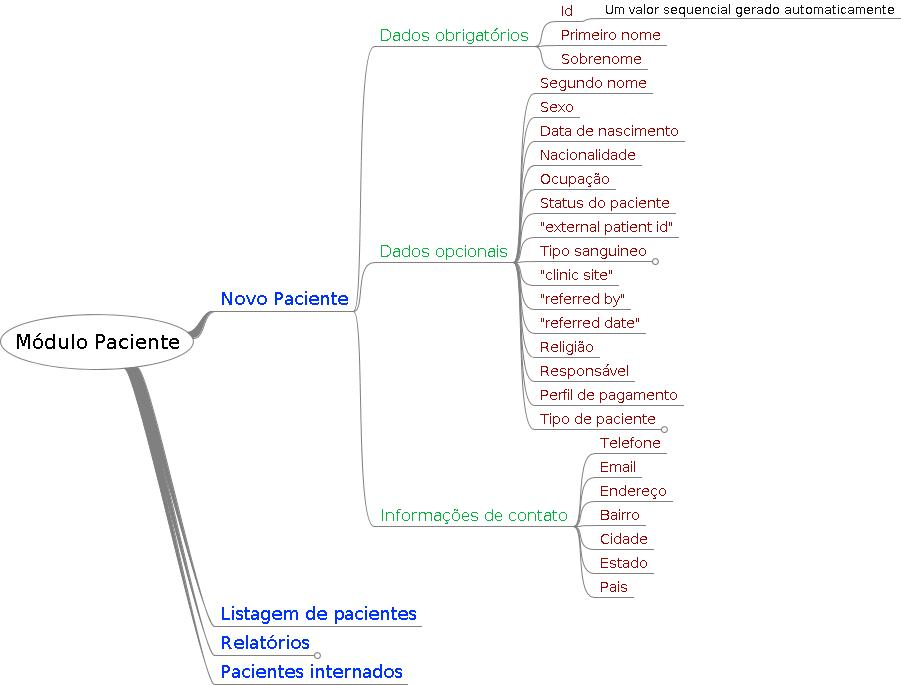
\includegraphics[scale=0.5]{map.jpeg}%\\[1cm] 

\section*{Análise de domínio}
\addcontentsline{toc}{section}{\protect\numberline{}Análise de domínio}

\paragraph{Variável ID}
\begin{itemize}
\item Nome da variável: ID
\item Dimensão primária: É uma string que serve como identificador único para
    cada paciente
\item Tipo da variável: String
\item A variável é ordenável.
\item É uma variável de entrada gerada automaticamente. Seu valor não depende
    de outras variáveis
\item Atua como identificador do paciente
\item Variáveis relacionadas: Nenhuma
\end{itemize}
\section*{Tabela de equivalência}
\addcontentsline{toc}{section}{\protect\numberline{}Tabela de equivalência}
\end{document}
